\documentclass[compress]{beamer}
\usepackage{ifthen,verbatim}

\newcommand{\isnote}{}
\xdefinecolor{lightyellow}{rgb}{1.,1.,0.25}
\xdefinecolor{darkblue}{rgb}{0.1,0.1,0.7}

%% Uncomment this to get annotations
%% \def\notes{\addtocounter{page}{-1}
%%            \renewcommand{\isnote}{*}
%% 	   \beamertemplateshadingbackground{lightyellow}{white}
%%            \begin{frame}
%%            \frametitle{Notes for the previous page (page \insertpagenumber)}
%%            \itemize}
%% \def\endnotes{\enditemize
%% 	      \end{frame}
%%               \beamertemplateshadingbackground{white}{white}
%%               \renewcommand{\isnote}{}}

%% Uncomment this to not get annotations
\def\notes{\comment}
\def\endnotes{\endcomment}

\setbeamertemplate{navigation symbols}{}
\setbeamertemplate{headline}{\mbox{ } \hfill
\begin{minipage}{5.5 cm}
\vspace{-0.75 cm} \small
\end{minipage} \hfill
\begin{minipage}{4.5 cm}
\vspace{-0.75 cm} \small
\begin{flushright}
\ifthenelse{\equal{\insertpagenumber}{1}}{}{Jim Pivarski \hspace{0.2 cm} \insertpagenumber\isnote/\pageref{numpages}}
\end{flushright}
\end{minipage}\mbox{\hspace{0.2 cm}}\includegraphics[height=1 cm]{../cmslogo} \hspace{0.01 cm} \vspace{-1.05 cm}}

\newcommand{\s}[1]{{\mbox{\scriptsize #1}}}

\begin{document}
\begin{frame}
\vfill
\begin{center}
\textcolor{darkblue}{\Large A Simple Quirk Hunt Using HSCP Tools}

\vfill
\begin{columns}
\column{0.3\linewidth}
\begin{center}
\large
Jim Pivarski
\end{center}
\end{columns}

%% \begin{columns}
%% \column{0.3\linewidth}
%% \begin{center}
%% \scriptsize
%% {\it Fermilab}
%% \end{center}
%% \end{columns}

\vfill
 8 September, 2011

\end{center}
\end{frame}

%% \begin{notes}
%% \item This is the annotated version of my talk.
%% \item If you want the version that I am presenting, download the one
%% labeled ``slides'' on Indico (or just ignore these yellow pages).
%% \item The annotated version is provided for extra detail and a written
%% record of comments that I intend to make orally.
%% \item Yellow notes refer to the content on the {\it previous} page.
%% \item All other slides are identical for the two versions.
%% \end{notes}

\small

\begin{frame}
\frametitle{What are quirks?}

\begin{itemize}
\item A new $SU(N)'$ gauge group added to the Standard Model with:
\begin{itemize}
\item new fermons $Q$ with $100 \lesssim m_Q \lesssim 1000$~GeV/$c^2$: ``quirks''
\item strong interactions {\it below} the TeV scale, $\Lambda \ll m_Q$: ``infracolor''
\end{itemize}

\item Weird phenomenology: macro or mesoscopic strings (flux tubes)

\begin{columns}
\column{0.05\linewidth}

\column{0.35\linewidth}
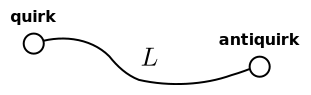
\includegraphics[width=\linewidth]{quirk_string.pdf}

\column{0.6\linewidth}
$\displaystyle L \sim \frac{m_Q}{\Lambda^2} \sim \mbox{10 m} \, \left(\frac{m_Q}{\mbox{TeV}}\right) \, \left(\frac{\Lambda}{\mbox{100 eV}}\right)^{-2}$
\end{columns}

\item \mbox{Kang \& Luty, {\it Macroscopic Strings and ``Quirks'' at Colliders} (2009)\hspace{-1 cm}} \\ \url{http://iopscience.iop.org/1126-6708/2009/11/065/} (arXiv:0805.4642), {\tiny see also cited-by: Quirky Dark Matter, SUSY quirks, and the $Wjj$ excess}

\end{itemize}

\vfill
\hspace{-0.83 cm} \textcolor{darkblue}{\Large Is this motivated by electroweak symmetry breaking/ the hierarchy problem/other theoretical problem?}

\begin{itemize}
\item No: it is a possibility that is consistent with known data, and might be missed without a deliberate search

\item Comparable to $Z'$, which is an extra $U(1)'$ that may or may not come from the breaking of a larger GUT group
\end{itemize}
\end{frame}

\begin{frame}
\frametitle{Signatures}

\hfill \includegraphics[width=3 cm]{diagram.png}

\vspace{-1.25 cm}
Infracolor string connecting quirks does not break, \\ so quirks orbit each other through the detector

\begin{center}
\includegraphics[width=0.7\linewidth]{weird_tracks.png}
\end{center}

\vspace{-0.5 cm}
\textcolor{darkblue}{This analysis:}
\begin{itemize}
\item Straight track from mesoscopic quirk string: \mbox{10~keV $\lesssim$ $\Lambda$ $\lesssim$ 1~MeV,\hspace{-0.5 cm}} quirks with electric charge but no QCD color
\end{itemize}

\textcolor{darkblue}{Other quirk signatures, not pursued here:}
\begin{itemize}
\item Tracks curving in $r$-$z$ plane: $\Lambda$ $\ll$ 10~keV

\item Free end of a string orbiting a stopped quirk (spiral track)

\item Hadronic fireball (many soft hadrons): quirks with QCD color

\item same with a displaced vertex: \mbox{\scriptsize $\displaystyle c\tau \sim \frac{m_Q}{\Lambda_\s{QCD}} \, \frac{m_Q}{\Lambda^2} \sim 100~\mu\mbox{m} \, \bigg(\frac{\Lambda}{\mbox{MeV}}\bigg)^{-2} \, \bigg(\frac{m_Q}{\mbox{TeV}}\bigg)^2$\hspace{-2 cm}}

\item Prompt annihilation or decay to infracolor glueballs: $\Lambda$ $\gg$ MeV
\end{itemize}
\end{frame}

\begin{frame}
\frametitle{Focus on the simplest signature}

\vspace{0.2 cm}
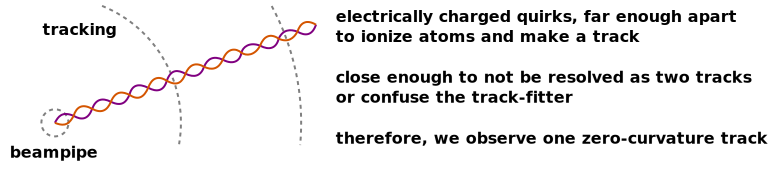
\includegraphics[width=\linewidth]{straight_track.pdf}

\begin{columns}
\column{0.6\linewidth}
\begin{itemize}
\item Unlike {\it all} backgrounds, the signal peaks at curvature = 0
\item If realistic distortions to curvature distribution can be quantified as nuisance parameters, search/limits can be performed with a fit (bump-hunt)
\end{itemize}
\column{0.4\linewidth}
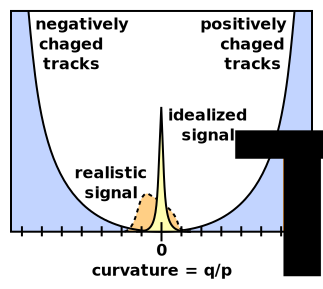
\includegraphics[width=\linewidth]{curvature_distribution.pdf}
\end{columns}

Since this object also has mass $\ge$ $2m_Q$, it will be slow ($\beta \ll 1$)
\begin{itemize}
\item Tracker $dE/dx$ and muon time-of-flight will be useful cuts
\item Mass varies event-by-event; it would not peak in HSCP mass plot
\end{itemize}
\end{frame}

\begin{frame}
\frametitle{Previous searches}

This technique was used by D\O\ (2.4~fb$^{-1}$, fall 2010)
\begin{itemize}
\item as a counting experiment, not bump-hunt
\item not triggered in muon system: associated with jet and $\not\!\!{E_{T}}$
\end{itemize}
\mbox{\url{http://prl.aps.org/abstract/PRL/v105/i21/e211803} (arXiv:1008.3547)\hspace{-1 cm}}

\vspace{0.2 cm}
\begin{columns}
\column{0.5\linewidth}
\centering D\O\ limits

\includegraphics[height=3.5 cm]{d0_limit.png}

\column{0.5\linewidth}
\centering Tevatron and LHC cross-sections

\includegraphics[height=3.5 cm]{production_crosssection.png}
\end{columns}

\vspace{0.2 cm}
\begin{itemize}
\item 95\% C.L.\ limits on quirk mass: 107, 119, 133~GeV/$c^2$ for $SU(2)'$, $SU(3)'$, $SU(5)'$, respectively (10~keV $<$ $\Lambda$ $<$ 1~MeV)
\item LHC ($E_\s{CM}$ = 10~TeV? 7~TeV?) can reach much higher in quirk mass
\end{itemize}
\end{frame}

\begin{frame}
\frametitle{Triggering}

\begin{itemize}
\item For $\beta > X$, quirk pair reaches the muon system within timing window: use highest-$p_T$ unprescaled single-muon trigger available
\begin{itemize}
\item \textcolor{gray}{1.5 bunch timing windows = 40~ns, muon system is 15~ns away from the beamspot, so $X = 0.4$?}
\item I do not yet know the $\beta$ distribution for this model at the LHC
\item At the Tevatron, $\beta$ distribution is ``very wide and peaks at $\beta$ $\sim$ 0.8 (0.2) for $m_Q$ = 60 (160) GeV/$c^2$'' (D\O\ paper)
\end{itemize}

\item For $\beta < X$, must trigger on the jet or photon that is produced with the quirk pair
\begin{itemize}
\item I don't know jet/photon distributions for the LHC yet, either
\item D\O\ analysis required exactly one $p_T > 75$~GeV/$c$ jet in $|\eta| < 1.6$ and $\not\!\!{E_{T}} > 50$~GeV

\end{itemize}
\end{itemize}

The single-muon trigger case is a subset of HSCP data, but the ``jet or photon'' is not (unless our calculation of $\not\!\!{E_{T}}$ excludes the HSCP track and we can expect large $\not\!\!{E_{T}}$)

\end{frame}

\begin{frame}
\frametitle{Monte Carlo}
\begin{itemize}
\item I'm writing to Markus Luty about using the same simulation as D\O
\begin{itemize}
\item $\beta$ distribution and associated jet or photon for trigger
\item classical trajectory and Bethe-Bloch $dE/dx$ for ionization
\end{itemize}

\item However, Tim Nelson and Jim Black (SLAC/ATLAS) are developing a
  much more realistic simulation of quirk propagation through matter: \mbox{\url{http://online.kitp.ucsb.edu/online/lhc11/nelson/}\hspace{-1 cm}}

\begin{center}
\includegraphics[width=0.27\linewidth]{23.jpg} \hspace{0.2 cm}
\includegraphics[width=0.27\linewidth]{24.jpg} \hspace{0.2 cm}
\includegraphics[width=0.27\linewidth]{25.jpg}

\includegraphics[width=0.27\linewidth]{26.jpg} \hspace{0.2 cm}
\includegraphics[width=0.27\linewidth]{27.jpg} % \hspace{0.2 cm}
% \includegraphics[width=0.27\linewidth]{28.jpg}
\end{center}

\item We should use this MC when it becomes available

\end{itemize}
\end{frame}

\begin{frame}
\frametitle{Future extensions}
\begin{itemize}
\item \mbox{Straight-track propagation is a special case in three important ways:\hspace{-1 cm}}
\begin{itemize}
\item infracolor string is required to be short compared to track hits
\item infracolor string is required to be long compared to atoms
\item quirks assumed to have zero QCD color
\end{itemize}

\item Three ways to generalize this analysis:
\begin{itemize}
\item expand track reconstruction to allow for curvature in the $r$-$z$ plane: this would allow for longer infracolor strings ($\Lambda < 10$~keV) and may double as a monopole search
\item search for hadronic fireballs and displaced fireballs: this would allow for quirks with QCD color (outside of HSCP group)
\item displaced dileptons and diphotons would capture the microscopic string case (partly covered elsewhere)
\end{itemize}

\item I only have resources to do the simple straight-track search

\item There are many more opportunities for people looking for a project
\end{itemize}
\end{frame}

\begin{frame}
\frametitle{Steps in the straight-track analysis}
\begin{enumerate}
\item Walk through Hscp2011Analysis twiki \hfill \textcolor{red}{(done)}

\item Obtain a quirk MC and integrate it into CMS (follow HSCP stau/stop/gluino examples to see how to add slow particles with large $dE/dx$? does Geant do this for us?)

\item Produce the analysis plot (curvature histogram, where signal peaks at zero) and {\it roughly} optimize cuts with MC

\item If a lot of the signal is out-of-time with the muon trigger, identify a good jet or photon trigger and produce a second sample

\item Use previously-studied trigger efficiency results (muon trigger as a function of $\beta$ and other triggers generically)

\item Calculate track-reconstruction efficiency as a function of infracolor string length (using Nelson and Black's realistic MC)

\item Study resolution of curvature = 0 peak from alignment and $Z \to \mu\mu$

\item Finalize cuts, fitting procedure, and limit/discovery procedure with MC and blinded data (blind in curvature and/or $dE/dx$)

\item Unblind and fit; write results as an independent Analysis Note and as a part of an upcoming HSCP paper
\end{enumerate}
\end{frame}

%% \begin{frame}
%% \frametitle{Outline}
%% \begin{itemize}\setlength{\itemsep}{0.75 cm}
%% \item 
%% \end{itemize}
%% %% \hspace{-0.83 cm} \textcolor{darkblue}{\Large Outline2}
%% \end{frame}

%% \section*{First section}
%% \begin{frame}
%% \begin{center}
%% \Huge \textcolor{blue}{First section}
%% \end{center}
%% \end{frame}

\begin{frame}
\frametitle{Conclusions}

\begin{itemize}\setlength{\itemsep}{0.25 cm}
\item Quirks are a possible extension of the Standard Model with bizarre~(fun) phenomenology
\item As far as I'm aware, there are no quirk analyses in CMS
\begin{itemize}
\item searching for ``quirks'' in HyperNews and Indico only result in messages about computer problems
\item in several old talks, Albert de Roeck tried to raise interest
\end{itemize}
\item The straight-track signature is {\it almost} a special case of the HSCP analysis; I think it should be presented as such
\item There are many other quirky signatures to look for
\end{itemize}
\label{numpages}
\end{frame}

\end{document}
